\documentclass[a4paper,10pt]{article}
\usepackage{pdfpages} 
\usepackage[dutch]{babel}
\usepackage[utf8]{inputenc}
\usepackage[official]{eurosym}
\usepackage{listings}
\usepackage[titles]{tocloft}
\usepackage{amssymb,amsmath}
\usepackage[nottoc, numbib]{tocbibind}
\usepackage{gensymb}
\usepackage{placeins}
\usepackage{float}
 
\title{Quantified Bike}
\author{Laurent Dossche \and Jakob Festraets \and Peter Lacko}
\date{27/11/2014}

\pdfinfo{%
  /Title    (Case Mechanica)
  /Author   (Laurent Dossche, Jakob Festraets, Peter Lacko)
  /Creator  ()
  /Producer ()
  /Subject  ()
  /Keywords ()
}
\setlength{\footskip}{100pt}
\begin{document}

%%%%%%%%%%%%%%%%%%%%%%%%%%%%%%%%%%%%%%%%%
% University Assignment Title Page 
% LaTeX Template
% Version 1.0 (27/12/12)
%
% This template has been downloaded from:
% http://www.LaTeXTemplates.com
%
% Original author:
% WikiBooks (http://en.wikibooks.org/wiki/LaTeX/Title_Creation)
%
% License:
% CC BY-NC-SA 3.0 (http://creativecommons.org/licenses/by-nc-sa/3.0/)
% 
% Instructions for using this template:
% This title page is capable of being compiled as is. This is not useful for 
% including it in another document. To do this, you have two options: 
%
% 1) Copy/paste everything between \begin{document} and \end{document} 
% starting at \begin{titlepage} and paste this into another LaTeX file where you 
% want your title page.
% OR
% 2) Remove everything outside the \begin{titlepage} and \end{titlepage} and 
% move this file to the same directory as the LaTeX file you wish to add it to. 
% Then add \input{./title_page_1.tex} to your LaTeX file where you want your
% title page.
%
%%%%%%%%%%%%%%%%%%%%%%%%%%%%%%%%%%%%%%%%%

%----------------------------------------------------------------------------------------
%	PACKAGES AND OTHER DOCUMENT CONFIGURATIONS
%----------------------------------------------------------------------------------------

\begin{titlepage}

\newcommand{\HRule}{\rule{\linewidth}{0.5mm}} % Defines a new command for the horizontal lines, change thickness here

\center % Center everything on the page
 
%----------------------------------------------------------------------------------------
%	HEADING SECTIONS
%----------------------------------------------------------------------------------------

\textsc{\LARGE ku leuven}\\[1.5cm] % Name of your university/college
\textsc{\Large Toegepaste Mechanica 2}\\[0.5cm] % Major heading such as course name
\textsc{\large Deel Dynamica}\\[0.5cm] % Minor heading such as course title

%----------------------------------------------------------------------------------------
%	TITLE SECTION
%----------------------------------------------------------------------------------------

\HRule \\[0.4cm]
{ \huge \bfseries CASE 2014-2015}\\[0.4cm] % Title of your document
\HRule \\[1.5cm]
 
%----------------------------------------------------------------------------------------
%	AUTHOR SECTION
%----------------------------------------------------------------------------------------

\begin{minipage}{0.4\textwidth}
\begin{flushleft} \large
\emph{Auteurs:}\\
Laurent \textsc{Dossche}\\ % Your name
Jakob \textsc{Festraets}\\
Peter \textsc{Lacko}
\end{flushleft}
\end{minipage}
~
\begin{minipage}{0.4\textwidth}
\begin{flushright} \large
\emph{Begeleiders:} \\
Wim \textsc{Desmet}\\ % Supervisor's Name
Jos \textsc{Vander Sloten}
\end{flushright}
\end{minipage}\\[4cm]

% If you don't want a supervisor, uncomment the two lines below and remove the section above
%\Large \emph{Author:}\\
%John \textsc{Smith}\\[3cm] % Your name

%----------------------------------------------------------------------------------------
%	DATE SECTION
%----------------------------------------------------------------------------------------

{\large 27 november 2014}\\[3cm] % Date, change the \today to a set date if you want to be precise

%----------------------------------------------------------------------------------------
%	LOGO SECTION
%----------------------------------------------------------------------------------------

%\includegraphics{Logo}\\[1cm] % Include a department/university logo - this will require the graphicx package
 
%----------------------------------------------------------------------------------------

\vfill % Fill the rest of the page with whitespace

\end{titlepage}

\newpage
\tableofcontents

\newpage
\section{Groepsleden}
Onze groep bestaat uit de volgende leden.
\begin{enumerate}
 \item Laurent DOSSCHE, Bachelor in de ingenieurswetenschappen, 2de jaar.
 \item Jakob FESTRAETS, Bachelor in de ingenieurswetenschappen, 2de jaar.
 \item Peter LACKO, Bachelor in de ingenieurswetenschappen, 2de jaar.
\end{enumerate}

\section{Transformatiematrices}
\begin{itemize}
\item De matrix in \eqref{eq:tm1} is de transformatiematrix om coördinaten van het bewegend $x'y'z'$-assenstelsel naar het wereldassenstelsel om te zetten. Dit bewegend assenstelsel heeft een draaing met een hoek $\alpha$ rond de x-as.
\begin{equation}
R^{x'y'z' \rightarrow xyz}=
\begin{bmatrix}
1			&			0			&			0		   \\
0			&\cos(\alpha)&-\sin(\alpha)\\
0			&\sin(\alpha)&\cos(\alpha) \\
\end{bmatrix}
\label{eq:tm1}
\end{equation}
\item Het $x''y''z''$-assenstelsel heeft dezelfde oriëntatie als het $x'y'z'$-assenstelsel. Hier is dus geen transformatiematrix vereist.
\item De matrix in \eqref{eq:tm2} is de transformatiematrix om coördinaten van het $x'''y'''z'''$-assenstelsel naar het $x''y''z''$-assenstelsel om te zetten. Dit eerste bewegend assenstelsel heeft een draaing met een hoek $\beta$ rond de x-as.
\begin{equation}
R^{x'''y'''z''' \rightarrow x''y''z''}=
\begin{bmatrix}
\cos(\beta)	&			0			&\sin(\beta)\\
0						&			1			&			0		 \\
-\sin(\beta)&			0			&\cos(\beta)\\
\end{bmatrix}
\label{eq:tm2}
\end{equation}
\item Het $x''''y''''z''''$-assenstelsel heeft dezelfde oriëntatie als het $x'''y'''z'''$-assenstelsel. Hier is dus geen transformatiematrix vereist.
\item De matrix in \eqref{eq:tm3} is de transformatiematrix om coördinaten van het $x'''y'''z'''$-assenstelsel of van het $x''''y''''z''''$-assenstelsel naar het wereldassenstelsel ($xyz$) om te zetten. Hierbij worden de coördinaten eerst omgezet naar het $x'y'z'$-assenstelsel en pas daarna naar het wereldassenstelsel. Dit kan met volgende matrixvermenigvuldiging.
\begin{equation}
\begin{split}
R^{x'''y'''z''' \rightarrow xyz}&=R^{x'y'z' \rightarrow xyz} \cdot R^{x'''y'''z''' \rightarrow x''y''z''}\\
&=
\begin{bmatrix}
1			&			0			&			0		   \\
0			&\cos(\alpha)&-\sin(\alpha)\\
0			&\sin(\alpha)&\cos(\alpha) \\
\end{bmatrix}
\cdot
\begin{bmatrix}
\cos(\beta)	&			0			&\sin(\beta)\\
0						&			1			&			0		 \\
-\sin(\beta)&			0			&\cos(\beta)\\
\end{bmatrix}\\
&=\begin{bmatrix}
\cos(\beta)							&			0				&\sin(\beta)\\
\sin(\alpha)\sin(\beta)	&\cos(\alpha)	&-\sin(\alpha)\cos(\beta)\\
-\cos(\alpha)\sin(\beta)&\sin(\alpha)	&\cos(\alpha)\cos(\beta)\\
\end{bmatrix}
\end{split}
\label{eq:tm3}
\end{equation}
\item De transpose van bovenstaande matrices geeft vanzelfsprekend de transformatiematrices om coördinaten in de omgekeerde richting te transformeren.
\end{itemize}
\section{Kinematica}
\subsection{Opgave 1}
\subsubsection{Rotatiesnelheid}
Om de ogenblikkelijke totale rotatiesnelheidsvector $\vec{\omega}_{tot}$ te berekenen zetten we eerst alle rotatiesnelheidsvectoren om naar het $x'y'z'$-assenstelsel. $\vec{\omega}_{g}$ en $\vec{\omega}_{i}$ staan hier al in, dus we moeten enkel $\vec{\omega}_{w}$ nog omzetten. 
\begin{equation}
\begin{split}
\vec{\omega}_{w}^{'}&=R^{x'''y'''z''' \rightarrow x'y'z'} \cdot \vec{\omega}_{w}^{'''}\\
&=\begin{bmatrix}
\cos(\beta)	&			0			&\sin(\beta)\\
0						&			1			&			0		 \\
-\sin(\beta)&			0			&\cos(\beta)\\
\end{bmatrix}
\cdot
\begin{bmatrix}
-\omega_{w}	\\
0						\\
0						\\
\end{bmatrix}\\
&=
\begin{bmatrix}
-\omega_{w}\cdot \cos(\beta)	\\
0						\\
\omega_{w}\cdot \sin(\beta)	\\
\end{bmatrix}
\end{split}
\label{eq:kin1.1}
\end{equation}
Als we al deze vectoren optellen krijgen we $\vec{\omega}_{tot}^{'}$\footnote{Notatie: het aantal accenten als superscript bij vectoren duidt op het assenstelsel waar de vector in is uitgedrukt.}
\begin{equation}
\begin{split}
\vec{\omega}_{tot}^{'}&=\vec{\omega}_{g}^{'} + \vec{\omega}_{i}^{'} + \vec{\omega}_{w}^{'}\\
&=\begin{bmatrix}
0						\\
0						\\
\omega_{g}	\\
\end{bmatrix}
+\begin{bmatrix}
0						\\
\omega_{i}	\\
0						\\
\end{bmatrix}
+\begin{bmatrix}
-\omega_{w}\cdot \cos(\beta)	\\
0						\\
\omega_{w}\cdot \sin(\beta)	\\
\end{bmatrix}\\
&=\begin{bmatrix}
-\omega_{w}\cdot \cos(\beta)	\\
\omega_{i}						\\
\omega_{g}+\omega_{w}\cdot \sin(\beta)	\\
\end{bmatrix}
\end{split}
\label{eq:kin1.2}
\end{equation}
Na omvorming naar het wereldassenstelsel krijgen we de ogenblikkelijke totale rotatiesnelheidsvector $\vec{\omega}_{tot}$.
\begin{equation}
\begin{split}
\vec{\omega}_{tot}&=R^{x'y'z' \rightarrow xyz} \cdot \vec{\omega}_{tot}^{'}\\
&=\begin{bmatrix}
1			&			0			&			0		   \\
0			&\cos(\alpha)&-\sin(\alpha)\\
0			&\sin(\alpha)&\cos(\alpha) \\
\end{bmatrix}
\cdot
\begin{bmatrix}
-\omega_{w}\cdot \cos(\beta)	\\
\omega_{i}						\\
\omega_{g}+\omega_{w}\cdot \sin(\beta)	\\
\end{bmatrix}\\
&=
\begin{bmatrix}
-\omega_{w}\cdot \cos(\beta)	\\
\omega_{i}\cos(\alpha)-\sin(\alpha)(\omega_{g}+\omega_{w}\sin(\beta))\\
\omega_{i}\sin(\alpha)+\cos(\alpha)(\omega_{g}+\omega_{w}\sin(\beta))\\
\end{bmatrix}
\end{split}
\label{eq:kin1.3}
\end{equation}
\newpage
\subsubsection{Rotatieversnelling}
Om de ogenblikkelijke totale rotatieversnellingsvector $\vec{\alpha}_{tot}$ te berekenen maken we gebruik van formule \eqref{eq:kin1.4}.
\begin{equation}
\vec{\alpha} = \sum_{i=1}^{k}{\frac{\mathrm{d}\omega_{i}}{\mathrm{d}t}\vec{e}_{\omega_{i}}}+\sum_{i=1}^{k}{\vec{\omega}_{i}\frac{\mathrm{d}\vec{e}_{\omega_{i}}}{\mathrm{d}t}}  
\label{eq:kin1.4}
\end{equation}
met:
\begin{equation}
\vec{\omega}_{i}\frac{\mathrm{d}\vec{e}_{\omega_{i}}}{\mathrm{d}t}=\sum_{j=1}^{i-1}{\vec{\omega}_{j}\times\vec{\omega}_{i}}  
\label{eq:kin1.5}
\end{equation}
Concreet wordt dit:
\begin{equation}
\vec{\alpha}_{tot} = \vec{\alpha}_{g} + \vec{\alpha}_{i} + \vec{\alpha}_{w} + \vec{\omega}_{g} \times \vec{\omega}_{i} + \vec{\omega}_{g} \times \vec{\omega}_{w} + \vec{\omega}_{i} \times \vec{\omega}_{w}
\label{eq:kin1.6}
\end{equation}
$\vec{\omega}_{g} \times \vec{\omega}_{w}$ en $\vec{\omega}_{i} \times \vec{\omega}_{w}$ zijn termen die duiden op de verandering van oriëntatie van $\vec{\omega}_{w}$. Zijn oriëntatie in namelijk is afhankelijk van $\vec{\omega}_{g}$ en $\vec{\omega}_{i}$. $\vec{\omega}_{g} \times \vec{\omega}_{i}$ is om dezelfde reden toegevoegd.

$\vec{\alpha}_{g}$, $\vec{\alpha}_{i}$, $\vec{\omega}_{g}$ en $\vec{\omega}_{i}$ zijn reeds uitgedrukt in het $x'y'z'$-assenstelsel. $\vec{\omega}_{w}$ werd al in \eqref{eq:kin1.1} naar dit assenstelsel getransformeerd. Hieronder wordt $\vec{\alpha}_{w}$ getransformeerd.
\begin{equation}
\begin{split}
\vec{\alpha}_{w}^{'}&=R^{x'''y'''z''' \rightarrow x'y'z'} \cdot \vec{\alpha}_{w}^{'''}\\
&=\begin{bmatrix}
\cos(\beta)	&			0			&\sin(\beta)\\
0						&			1			&			0		 \\
-\sin(\beta)&			0			&\cos(\beta)\\
\end{bmatrix}
\cdot
\begin{bmatrix}
\alpha_{w}	\\
0						\\
0						\\
\end{bmatrix}\\
&=
\begin{bmatrix}
\alpha_{w}\cdot \cos(\beta)	\\
0						\\
-\alpha_{w}\cdot \sin(\beta)	\\
\end{bmatrix}
\end{split}
\label{eq:kin1.7}
\end{equation}
Uitgewerkt wordt $\vec{\alpha}_{tot}$:
\begin{equation}
\begin{split}
\vec{\alpha}_{tot}^{'} &= \vec{\alpha}_{g}^{'} + \vec{\alpha}_{i}^{'} + \vec{\alpha}_{w}^{'} + \vec{\omega}_{g}^{'} \times \vec{\omega}_{i}^{'} + \vec{\omega}_{g}^{'} \times \vec{\omega}_{w}^{'} + \vec{\omega}_{i}^{'} \times \vec{\omega}_{w}^{'}\\
&=\begin{bmatrix}
0						\\
0						\\
\alpha_{g}	\\
\end{bmatrix}
+\begin{bmatrix}
0						\\
\alpha_{i}	\\
0						\\
\end{bmatrix}
+\begin{bmatrix}
\alpha_{w}\cdot \cos(\beta)	\\
0						\\
-\alpha_{w}\cdot \sin(\beta)	\\
\end{bmatrix}
+\begin{vmatrix}
e_{x}&e_{y}&e_{z}\\
0&0&\omega_{g}\\
0&\omega_{i}&0\\
\end{vmatrix}\\
&+\begin{vmatrix}
e_{x}&e_{y}&e_{z}\\
0&0&\omega_{g}\\
-\omega_{w}\cdot \cos(\beta)&0&\omega_{w}\cdot \sin(\beta)\\
\end{vmatrix}
+\begin{vmatrix}
e_{x}&e_{y}&e_{z}\\
0&\omega_{i}&0\\
-\omega_{w}\cdot \cos(\beta)&0&\omega_{w}\cdot \sin(\beta)\\
\end{vmatrix}\\
&=\begin{bmatrix}
\alpha_{w}\cos(\beta)-\omega_{i}\omega_{g}+\omega_{i}\omega_{w}\sin{\beta}\\
\alpha_{i}-\omega_{g}\omega_{w}\cos{\beta}\\
\alpha_{g}-	\alpha_{w} \sin(\beta)+\omega_{i}\omega_{w}\cos{\beta}\\
\end{bmatrix}
\label{eq:kin1.8}
\end{split}
\end{equation}
\begin{equation}
\begin{split}
\vec{\alpha}_{tot}&=R^{x'y'z' \rightarrow xyz} \cdot \vec{\alpha}_{tot}^{'}\\
&=\begin{bmatrix}
1			&			0			&			0		   \\
0			&\cos(\alpha)&-\sin(\alpha)\\
0			&\sin(\alpha)&\cos(\alpha) \\
\end{bmatrix}
\cdot
\begin{bmatrix}
-\alpha_{w}\cos(\beta)-\omega_{i}\omega_{g}+\omega_{i}\omega_{w}\sin{\beta}\\
\alpha_{i}-\omega_{g}\omega_{w}\cos{\beta}\\
\alpha_{g}+	\alpha_{w} \sin(\beta)+\omega_{i}\omega_{w}\cos{\beta}\\
\end{bmatrix}
\end{split}
\label{eq:kin1.9}
\end{equation}
De uitwerking wordt hier achterwege gelaten wegens te complex.
\newpage
\subsection{Opgave 2}
\subsubsection{Snelheid}
Om de ogenblikkelijke snelheid $\vec{v}_{c}$ van het punt C te berekenen hebben wij voor een combinatie van methodes gekozen. Ten eerste is er een samengestelde beweging met het $x'y'z'$-assenstelsel als bewegend assenstelsel. Hierdoor heeft de sleepsnelheid in \eqref{eq:kin2.6} een component veroorzaakt door de translatie van het vliegtuig met snelheid $\vec{v}_{v}$ en een component veroorzaakt door de rotatie van het vliegtuig met rotatiesnelheid $\vec{\omega}_{g}$. Ten tweede maken we gebruik van de methode van som van rotaties om de relatieve snelheid in \eqref{eq:kin2.7} van de eerder vermelde samengestelde beweging te berekenen. We moeten eerst echter de afstandsvectoren berekenen.
\begin{equation}
\vec{r}_{AB}^{'}=
\begin{bmatrix}
l_{1}\\
0\\
l_{2}\\
\end{bmatrix}
\label{eq:kin2.3}
\end{equation}
\begin{equation}
\vec{r}_{BC}^{'}=
\begin{bmatrix}
-(l_{3}\sin{\beta}+l_{4}\cos{\beta})\\
0\\
-l_{3}\cos{\beta}+l_{4}\sin{\beta}\\
\end{bmatrix}
\label{eq:kin2.4}
\end{equation}
\begin{equation}
\vec{r}_{AC}^{'}=
\begin{bmatrix}
l_{1}-(l_{3}\sin{\beta}+l_{4}\cos{\beta})\\
0\\
l_{2}-l_{3}\cos{\beta}+l_{4}\sin{\beta}\\
\end{bmatrix}
\label{eq:kin2.5}
\end{equation}
De sleepsnelheid uitgedrukt in het $x'y'z'$-assenstelsel.
\begin{equation}
\begin{split}
\vec{v}_{sleep}^{'}&=\vec{v}_{v}^{'}+\vec{\omega}_{g}^{'}\times\vec{r}_{AC}^{'}\\
&=\begin{bmatrix}
0						\\
v_{v}	\\
0						\\
\end{bmatrix}
+\begin{vmatrix}
e_{x}&e_{y}&e_{z}\\
0&0&\omega_{g}\\
l_{1}-(l_{3}\sin{\beta}+l_{4}\cos{\beta})&0&l_{2}-l_{3}\cos{\beta}+l_{4}\sin{\beta}\\
\end{vmatrix}\\
&=\begin{bmatrix}
0						\\
v_{v}+\omega_{g}\,\left( l_{1}-\cos \left( \beta \right) l_{4}-\sin \left( \beta \right) l_{3} \right)\\
0						\\
\end{bmatrix}
\end{split}
\label{eq:kin2.6}
\end{equation}
Ook de relatieve snelheid wordt in het $x'y'z'$-assenstelsel uitgedrukt. $\vec{\omega}_{w}$ is niet opgenomen in de formule omdat deze geen bijdrage bij de snelheid van C levert.
\begin{equation}
\begin{split}
\vec{v}_{rel}^{'}&=\vec{\omega}_{i}^{'}\times\vec{r}_{BC}^{'}\\
&=\begin{vmatrix}
e_{x}&e_{y}&e_{z}\\
0&\omega_{i}&0\\
-(l_{3}\sin{\beta}+l_{4}\cos{\beta})&0&-l_{3}\cos{\beta}+l_{4}\sin{\beta}\\
\end{vmatrix}\\
&=\left[ \begin {array}{c} \omega_{i}\, \left( \sin \left( \beta
 \right) l_{4}-\cos \left( \beta \right) l_{3} \right)\\ 0\\-\omega_{i}\, \left( -\cos \left( \beta \right) l_{4}-\sin \left( \beta \right) l_{3} \right)\end {array} \right]
\end{split}
\label{eq:kin2.7}
\end{equation}
Na optelling van de sleepsnelheid en relatieve snelheid bekomen we \eqref{eq:kin2.8}.
\begin{equation}
\vec{v}_{c}^{'}=\left[ \begin {array}{c} \omega_{i}\, \left( \sin \left( \beta
 \right) l_{4}-\cos \left( \beta \right) l_{3} \right) 
\\ \noalign{\medskip}-\cos \left( \beta \right) l_{4}\,\omega_{g}-\sin
 \left( \beta \right) l_{3}\,\omega_{g}+l_{1}\,\omega_{g}+v_{v}
\\ \noalign{\medskip}\omega_{i}\, \left( \cos \left( \beta \right) l_{
4}+\sin \left( \beta \right) l_{3} \right) \end {array} \right]
\label{eq:kin2.8}
\end{equation}
\newpage
\subsubsection{Versnelling}
\label{sec:versnelling}
De versnelling wordt op dezelfde manier bepaald. We nemen opnieuw het $x'y'z'$-assenstelsel als bewegend assenstelsel voor de samengestelde beweging.
\begin{equation}
\vec{a}_{tot}^{'}=\vec{a}_{sleep}^{'}+\vec{a}_{rel}^{'}+\vec{a}_{comp}^{'}
\label{eq:kin2.9}
\end{equation}
met:
\begin{equation}
\begin{split}
\vec{a}_{sleep}^{'}&=\vec{a}_{v}^{'}+\vec{\alpha}_{g}^{'}\times\vec{r}_{AC}^{'}+\vec{\omega}_{g}^{'}\times(\vec{v}_{c}^{'}-\vec{v}_{a}^{'})\\
&=\begin{bmatrix}
0						\\
\alpha_{v}	\\
0						\\
\end{bmatrix}
+\begin{vmatrix}
e_{x}&e_{y}&e_{z}\\
0&0&\alpha_{g}\\
l_{1}-(l_{3}\sin{\beta}+l_{4}\cos{\beta})&0&l_{2}-l_{3}\cos{\beta}+l_{4}\sin{\beta}\\
\end{vmatrix}\\
&+\begin{vmatrix}
e_{x}&e_{y}&e_{z}\\
0&0&\omega_{g}\\
\omega_{i}\, \left( \sin \left( \beta \right) l_{4}-\cos \left( \beta \right) l_{3} \right)&\omega_{g}\, \left( l_{1}-\cos \left( \beta \right) l_{4}-\sin \left( \beta \right) l_{3} \right)&-\omega_{i}\, \left( -\cos \left( \beta \right) l_{4}-\sin \left( \beta \right) l_{3} \right)\\
\end{vmatrix}\\
&=\left[ \begin {array}{c} -{\omega_{g}}^{2} \left( l_{1}-\cos \left( \beta \right) l_{4}-\sin \left( \beta \right) l_{3} \right) 
\\a_{v}+\alpha_{g}\, \left( l_{1}-\cos \left( \beta \right) l_{4}-\sin \left( \beta \right) l_{3} \right) +\omega_{g}\,\omega_{i}\, \left( \sin \left( \beta \right) l_{4}-\cos \left( \beta \right) l_{3} \right) \\0\end {array} \right] 
\label{eq:kin2.10}
\end{split}
\end{equation}
\begin{equation}
\begin{split}
\vec{a}_{rel}^{'}&=\vec{\alpha}_{i}^{'}\times\vec{r}_{BC}^{'}+\vec{\omega}_{i}^{'}\times(\vec{v}_{c}^{'}-\vec{v}_{b}^{'})\\
&=\begin{vmatrix}
e_{x}&e_{y}&e_{z}\\
0&\alpha_{i}&0\\
-(l_{3}\sin{\beta}+l_{4}\cos{\beta})&0&-l_{3}\cos{\beta}+l_{4}\sin{\beta}\\
\end{vmatrix}\\
&+\begin{vmatrix}
e_{x}&e_{y}&e_{z}\\
0&\omega_{i}&0\\
\omega_{i}(\sin{\beta}l_{4}-\cos{\beta}l_{3})&-\omega_{g}(\cos{\beta}l_{4}+\sin{\beta}l_{3})&\omega_{i}(\cos{\beta}l_{4}+\sin{\beta}l_{3})\\
\end{vmatrix}\\
&=\left[ \begin {array}{c} \alpha_{i}\, \left( \sin \left( \beta
 \right) l_{4}-\cos \left( \beta \right) l_{3} \right) -{\omega_{i}}^{2} \left( -\cos \left( \beta \right) l_{4}-\sin \left( \beta \right) l_{3} \right) \\0\\ -\alpha_{i}\, \left( -\cos \left( \beta \right) l_{4}-\sin \left( \beta \right) l_{3} \right) -{\omega_{i}}^{2} \left( \sin \left( \beta \right) l_{4}-
\cos \left( \beta \right) l_{3} \right) \end {array} \right]
\end{split}
\label{eq:kin2.11}
\end{equation}
\begin{equation}
\begin{split}
\vec{a}_{comp}^{'}&=2\cdot(\vec{\omega}_{g}^{'}\times\vec{v}_{rel}^{'})\\
&=2\cdot
\begin{vmatrix}
e_{x}&e_{y}&e_{z}\\
0&0&\omega_{g}\\
\omega_{i}(\sin(\beta)l_{4}-\cos(\beta)l_{3})&0&\omega_{i}(\cos(\beta)l_{4}+\sin(\beta)l_{3})\\
\end{vmatrix}\\
&=\left[ \begin {array}{c} 0\\2\,\omega_{g}\,\omega_
{i}\, \left( \sin \left( \beta \right) l_{4}-\cos \left( \beta
 \right) l_{3} \right) \\ 0\end {array} \right]
\end{split}
\label{eq:kin2.12}
\end{equation}
Hieronder worden nog enkele termen van bovenstaande formules nader verklaard:
\begin{itemize}
\item In de derde term van de sleepsnelheid staat $\vec{v}_{c}^{'}-\vec{v}_{a}^{'}$. Hierbij is $\vec{v}_{c}^{'}$ de snelheid van het punt C dat in \eqref{eq:kin2.8} al berekend werd. $\vec{v}_{a}^{'}$ is de snelheid van het punt waar $vec{\omega}_{g}$ aangrijpt. In dit geval punt A. De snelheid van punt A is gelijk aan $\vec{v}_{v}^{'}$. 
\begin{equation}
\vec{v}_{c}^{'}-\vec{v}_{a}^{'}=\vec{v}_{c}^{'}-\vec{v}_{v}^{'}=
\left[ \begin {array}{c} \omega_{i}\, \left( \sin \left( \beta
 \right) l_{4}-\cos \left( \beta \right) l_{3} \right) 
\\ \noalign{\medskip}\omega_{g}\, \left( l_{1}-\cos \left( \beta
 \right) l_{4}-\sin \left( \beta \right) l_{3} \right) 
\\ \noalign{\medskip}\omega_{i}\, \left( \cos \left( \beta \right) l_{4}+\sin \left( \beta \right) l_{3} \right) \end {array} \right]
\label{eq:kin2.13}
\end{equation}
\item De tweede term van de relatieve snelheid bevat de snelheid van het punt B. Die wordt hieronder in detail uitgewerkt.
\begin{equation}
\begin{split}
\vec{v}_{b}^{'}&=\vec{v}_{v}^{'}+\vec{\omega}_{g}^{'}\times\vec{r}_{AB}^{'}\\
&=\begin{bmatrix}
0\\
v_{v}\\
0\\
\end{bmatrix}
+\begin{vmatrix}
e_{x}&e_{y}&e_{z}\\
0&0&\omega_{g}\\
l_{1}&0&l_{2}\\
\end{vmatrix}\\
&=\begin{bmatrix}
0\\
v_{v}+l_{1}\omega_{g}\\
0\\
\end{bmatrix}
\label{eq:kin2.14}
\end{split}
\end{equation}
\end{itemize}
Als we formule \eqref{eq:kin2.10},\eqref{eq:kin2.11} en \eqref{eq:kin2.12} in \eqref{eq:kin2.9} invullen krijgen we:
\begin{equation}
\vec{a}_{tot}^{'}=\left[ \begin {array}{c} -{\omega_{g}}^{2} \left( l_{1}-\cos \left( 
\beta \right) l_{4}-\sin \left( \beta \right) l_{3} \right) +\alpha_{i
}\, \left( \sin \left( \beta \right) l_{4}-\cos \left( \beta \right) l
_{3} \right) -{\omega_{i}}^{2} \left( -\cos \left( \beta \right) l_{4}
-\sin \left( \beta \right) l_{3} \right) \\ \noalign{\medskip}a_{v}+
\alpha_{g}\, \left( l_{1}-\cos \left( \beta \right) l_{4}-\sin \left( 
\beta \right) l_{3} \right) +3\,\omega_{g}\,\omega_{i}\, \left( \sin
 \left( \beta \right) l_{4}-\cos \left( \beta \right) l_{3} \right) 
\\ \noalign{\medskip}-\alpha_{i}\, \left( -\cos \left( \beta \right) l
_{4}-\sin \left( \beta \right) l_{3} \right) -{\omega_{i}}^{2} \left( 
\sin \left( \beta \right) l_{4}-\cos \left( \beta \right) l_{3}
 \right) \end {array} \right]
\label{eq:kin2.15}
\end{equation}
De volledige uitwerking naar het wereldassenstelsel zou te complex worden. Hieronder wordt dus louter de formule gegeven.
\begin{equation}
\vec{\alpha}_{tot}=R^{x'y'z' \rightarrow xyz}\cdot\vec{\alpha}_{tot}^{'}
\end{equation}
\newpage
\subsection{Opgave 3}
Zowel het $x'y'z'$-assenstelsel als het $x''y''z''$-assenstelsel zijn vast aan het vliegtuig gemonteerd. Dit heeft als gevolg dat de relatieve component van de snelheid van het punt C gelijk is met zowel het $x'y'z'$-assenstelsel als het $x''y''z''$-assenstelsel als bewegend assenstelsel. Dit geeft voor de versnelling dezelfde coriolis bijdrage als bij opgave 2.
\begin{equation}
\begin{split}
\vec{a}_{comp}^{'}&=2\cdot(\vec{\omega}_{g}^{'}\times\vec{v}_{rel}^{'})\\
&=2\cdot
\begin{vmatrix}
e_{x}&e_{y}&e_{z}\\
0&0&\omega_{g}\\
\omega_{i}(\sin(\beta)l_{4}-\cos(\beta)l_{3})&0&\omega_{i}(\cos(\beta)l_{4}+\sin(\beta)l_{3})\\
\end{vmatrix}\\
&=\left[ \begin {array}{c} 0\\2\,\omega_{g}\,\omega_
{i}\, \left( \sin \left( \beta \right) l_{4}-\cos \left( \beta
 \right) l_{3} \right) \\ 0\end {array} \right]
\end{split}
\label{eq:kin3.1}
\end{equation}
\subsection{Opgave 4}
\subsubsection{Snelheid}
Om de snelheid van het punt D te bepalen zullen we dezelfde werkwijze als bij opgave 2 hanteren (een combinatie van samengestelde beweging en som van rotaties). We beginnen echter met de afstandsvectoren.
\begin{equation}
\vec{r}_{AB}^{'}=
\begin{bmatrix}
l_{1}\\
0\\
l_{2}\\
\end{bmatrix}
\label{eq:kin4.1}
\end{equation}
\begin{equation}
\vec{r}_{BD}^{'}=
\begin{bmatrix}
\frac{3}{4} l_{4}\\
0\\
\frac{1}{4}l_{3}\\
\end{bmatrix}
\label{eq:kin4.2}
\end{equation}
\begin{equation}
\vec{r}_{AD}^{'}=
\begin{bmatrix}
l_{1}+\frac{3}{4}l_{4}\\
0\\
l_{2}+\frac{1}{4}l_{3}\\
\end{bmatrix}
\label{eq:kin4.3}
\end{equation}
De sleepsnelheid uitgedrukt in het $x'y'z'$-assenstelsel.
\begin{equation}
\begin{split}
\vec{v}_{sleep}^{'}&=\vec{v}_{v}^{'}+\vec{\omega}_{g}^{'}\times\vec{r}_{AD}^{'}\\
&=\begin{bmatrix}
0						\\
v_{v}	\\
0						\\
\end{bmatrix}
+\begin{vmatrix}
e_{x}&e_{y}&e_{z}\\
0&0&\omega_{g}\\
l_{1}+\frac{3}{4}l_{4}&0&l_{2}+\frac{1}{4}l_{3}\\
\end{vmatrix}\\
&=\begin{bmatrix}
0						\\
v_{v}+\omega_{g}\,\left( l_{1}+\frac{3}{4} l_{4}\right)\\
0						\\
\end{bmatrix}
\end{split}
\label{eq:kin4.4}
\end{equation}
Ook de relatieve snelheid wordt in het $x'y'z'$-assenstelsel uitgedrukt.
\begin{equation}
\begin{split}
\vec{v}_{rel}^{'}&=\vec{\omega}_{i}^{'}\times\vec{r}_{BD}^{'}\\
&=\begin{vmatrix}
e_{x}&e_{y}&e_{z}\\
0&\omega_{i}&0\\
\frac{3}{4}l_{4}&0&\frac{1}{4}l_{3}\\
\end{vmatrix}\\
&=\left[\begin{array}{c}\frac{1}{4}\,\omega_{i}\,l_{3}\\0\\-\frac{3}{4}\,\omega_{i}\,l_{4}\end{array}\right]
\end{split}
\label{eq:kin4.5}
\end{equation}
Na optelling van de sleepsnelheid en relatieve snelheid bekomen we \eqref{eq:kin4.6}.
\begin{equation}
\vec{v}_{d}^{'}=\left[ \begin {array}{c} 1/4\,\omega_{i}\,l_{3}\\ \noalign{\medskip}v_{v}+\omega_{g}\, \left( l_{1}+3/4\,l_{4} \right) \\ \noalign{\medskip}-3/4\,\omega_{i}\,l_{4}\end {array} \right]
\label{eq:kin4.6}
\end{equation}
\subsubsection{Versnelling}
De versnelling van het punt D wordt op volledig dezelfde manier bepaald als de versnelling van het punt C als in \ref{sec:versnelling}. Hieronder worden enkel de formules met hun uitwerking neergeschreven vermits de werkwijze eerder al werd verduidelijkt.
\begin{equation}
\begin{split}
\vec{a}_{sleep}^{'}&=\vec{a}_{v}^{'}+\vec{\alpha}_{g}^{'}\times\vec{r}_{AD}^{'}+\vec{\omega}_{g}^{'}\times(\vec{v}_{d}^{'}-\vec{v}_{a}^{'})\\
&=\begin{bmatrix}
0						\\
\alpha_{v}	\\
0						\\
\end{bmatrix}
+\begin{vmatrix}
e_{x}&e_{y}&e_{z}\\
0&0&\alpha_{g}\\
l_{1}+\frac{3}{4}l_{4}&0&l_{2}+\frac{1}{4}l_{3}\\
\end{vmatrix}\\
&+\begin{vmatrix}
e_{x}&e_{y}&e_{z}\\
0&0&\omega_{g}\\
\frac{1}{4}\,\omega_{i}\,l_{3}&\omega_{g}\, \left( l_{1}+\frac{3}{4}\,l_{4} \right)&-\frac{3}{4}\,\omega_{i}\,l_{4}\\
\end{vmatrix}\\
&=\left[ \begin {array}{c} -{\omega_{g}}^{2} \left( l_{1}+\frac{3}{4}\,l_{4} \right) \\a_{v}+\alpha_{g}\, \left( l_{1}+\frac{3}{4}\,l_{4} \right) +\frac{1}{4}\,\omega_{g}\,\omega_{i}\,l_{3}\\0\end {array} \right]
\label{eq:kin4.7}
\end{split}
\end{equation}
\begin{equation}
\begin{split}
\vec{a}_{rel}^{'}&=\vec{\alpha}_{i}^{'}\times\vec{r}_{BD}^{'}+\vec{\omega}_{i}^{'}\times(\vec{v}_{d}^{'}-\vec{v}_{b}^{'})\\
&=\begin{vmatrix}
e_{x}&e_{y}&e_{z}\\
0&\alpha_{i}&0\\
\frac{3}{4}l_{4}&0&\frac{1}{4}l_{3}\\
\end{vmatrix}\\
&+\begin{vmatrix}
e_{x}&e_{y}&e_{z}\\
0&\omega_{i}&0\\
\frac{1}{4}\,\omega_{i}\,l_{3}&\omega_{g}\, \left( l_{1}+\frac{3}{4}\,l_{4} \right)-l_{1}\,\omega_{g}&-\frac{3}{4}\,\omega_{i}\,l_{4}\\
\end{vmatrix}\\
&=\left[ \begin {array}{c} 1/4\,\alpha_{i}\,l_{3}-3/4\,{\omega_{i}}^{2}l_{4}\\0\\-3/4\,\alpha_{i}\,l_{4}-1/4\,{\omega_{i}}^{2}l_{3}\end {array} \right]
\end{split}
\label{eq:kin4.8}
\end{equation}
\begin{equation}
\begin{split}
\vec{a}_{comp}^{'}&=2\cdot(\vec{\omega}_{g}^{'}\times\vec{v}_{rel}^{'})\\
&=2\cdot
\begin{vmatrix}
e_{x}&e_{y}&e_{z}\\
0&0&\omega_{g}\\
\frac{1}{4}\,\omega_{i}\,l_{3}\\0\\-\frac{3}{4}\,\omega_{i}\,l_{4}\\
\end{vmatrix}\\
&=\left[ \begin {array}{c} 0\\ \frac{1}{2}\,\omega_{g}\,
\omega_{i}\,l_{3}\\ 0\end {array} \right]
\end{split}
\label{eq:kin4.9}
\end{equation}
\begin{equation}
\vec{v}_{d}^{'}-\vec{v}_{a}^{'}=\vec{v}_{d}^{'}-\vec{v}_{v}^{'}=
\left[ \begin {array}{c} \frac{1}{4}\,\omega_{i}\,l_{3}\\ \noalign{\medskip}\omega_{g}\, \left( l_{1}+\frac{3}{4}\,l_{4} \right) \\ \noalign{\medskip}-\frac{3}{4}\,\omega_{i}\,l_{4}\end {array} \right]
\label{eq:kin4.10}
\end{equation}
\begin{equation}
\begin{split}
\vec{v}_{b}^{'}&=\vec{v}_{v}^{'}+\vec{\omega}_{g}^{'}\times\vec{r}_{AB}^{'}\\
&=\begin{bmatrix}
0\\
v_{v}\\
0\\
\end{bmatrix}
+\begin{vmatrix}
e_{x}&e_{y}&e_{z}\\
0&0&\omega_{g}\\
l_{1}&0&l_{2}\\
\end{vmatrix}\\
&=\begin{bmatrix}
0\\
v_{v}+l_{1}\omega_{g}\\
0\\
\end{bmatrix}
\label{eq:kin4.11}
\end{split}
\end{equation}
De uiteindelijke oplossing:
\begin{equation}
\vec{a}_{tot}^{'}=\left[ \begin {array}{c} -{\omega_{g}}^{2} \left( l_{1}+\frac{3}{4}\,l_{4} \right) +\frac{1}{4} \,\alpha_{i}\,l_{3}-\frac{3}{4}\,{\omega_{i}}^{2}l_{4}\\ \noalign{\medskip}a_{v}+\alpha_{g}\, \left( l_{1}+\frac{3}{4}\,l_{4} \right) +\frac{3}{4}\,\omega_{g}\,\omega_{i}\,l_{3}\\ \noalign{\medskip}-\frac{3}{4}\,\alpha_{i}\,l_{4}-\frac{1}{4}\,{\omega_{i}}^{2}l_{3}\end {array} \right]
\label{eq:kin4.12}
\end{equation}
\begin{equation}
\vec{\alpha}_{tot}=R^{x'y'z' \rightarrow xyz}\cdot\vec{\alpha}_{tot}^{'}
\end{equation}
\newpage
\section{Dynamica}
\subsection{Opgave 1}
\subsubsection{Impuls}
De snelheid van het punt D en van het punt C die nodig is om de ogenblikkelijke impulsvector van het landingsgestel en het wiel te berekenen, werd al berekend in respectievelijk \eqref{eq:kin4.6} en \eqref{eq:kin2.8}.
\begin{itemize}
\item \textbf{Landingsgestel} 
\begin{equation}
\vec{p}_{l}^{'}=m_{l}\vec{v}_{d}^{'}=
\left[ \begin {array}{c} m_{l}\frac{1}{4}\,\omega_{i}\,l_{3}\\ \noalign{\medskip}m_{l}(v_{v}+\omega_{g}\, \left( l_{1}+\frac{3}{4}\,l_{4}) \right) \\ \noalign{\medskip}-m_{l}\frac{3}{4}\,\omega_{i}\,l_{4}\end {array} \right]
\label{eq:dyn1.1}
\end{equation}
\item \textbf{Wiel}
\begin{equation}
\vec{p}_{w}^{'}=m_{w}\vec{v}_{c}^{'}=
\left[ \begin {array}{c} m_{w}\omega_{i}\, \left( \sin \left( \beta
 \right) l_{4}-\cos \left( \beta \right) l_{3} \right) \\ \noalign{\medskip}m_{w}(-\cos \left( \beta \right) l_{4}\,\omega_{g}-\sin \left( \beta \right) l_{3}\,\omega_{g}+l_{1}\,\omega_{g}+v_{v})\\\noalign{\medskip}m_{w}\omega_{i}\, \left( \cos \left( \beta \right) l_{4}+\sin \left( \beta \right) l_{3} \right) \end {array} \right]
\label{eq:dyn1.2}
\end{equation}
\end{itemize}
\subsubsection{Verandering van impuls}
Ook de versnelling van de punten D en C zijn hier nodig en werden eerder al berekend in \eqref{eq:kin4.12} en \eqref{eq:kin2.15}.
\begin{itemize}
\item \textbf{Landingsgestel}
\begin{equation}
\frac{\mathrm{d}\vec{p}_{l}^{'}}{\mathrm{d}t}=m_{l}\vec{a}_{d}^{'}
=\left[ \begin {array}{c} m_{l}(-{\omega_{g}}^{2} \left( l_{1}+\frac{3}{4}\,l_{4} \right) +\frac{1}{4} \,\alpha_{i}\,l_{3}-\frac{3}{4}\,{\omega_{i}}^{2}l_{4})\\ \noalign{\medskip}m_{l}(a_{v}+\alpha_{g}\, \left( l_{1}+\frac{3}{4}\,l_{4} \right) +\frac{3}{4}\,\omega_{g}\,\omega_{i}\,l_{3})\\ \noalign{\medskip}m_{l}(-\frac{3}{4}\,\alpha_{i}\,l_{4}-\frac{1}{4}\,{\omega_{i}}^{2}l_{3})\end {array} \right]
\label{eq:dyn1.3}
\end{equation}
\item \textbf{Wiel}
\def\arraystretch{0.5}
\begin{equation}
\frac{\mathrm{d}\vec{p}_{w}^{'}}{\mathrm{d}t}=m_{w}\vec{a}_{c}^{'}
=\left[\begin{smallmatrix}m_{w}(-{\omega_{g}}^{2}\left(l_{1}-\cos\left(\beta\right)l_{4}-\sin\left(\beta\right)l_{3}\right)+\alpha_{i}\, \left(\sin\left(\beta\right)l_{4}-\cos\left(\beta\right)l_{3}\right)-{\omega_{i}}^{2}\left(-\cos\left(\beta\right)l_{4}-\sin \left(\beta\right)l_{3}\right))\\ \noalign{\medskip}m_{w}(a_{v}+\alpha_{g}\, \left( l_{1}-\cos \left( \beta \right) l_{4}-\sin \left(\beta\right)l_{3}\right)+3\,\omega_{g}\,\omega_{i}\,\left(\sin\left(\beta\right)l_{4}-\cos\left(\beta\right)l_{3}\right))\\ \noalign{\medskip}m_{w}(-\alpha_{i}\,\left(-\cos\left(\beta\right)l_{4}-\sin\left(\beta\right)l_{3}\right)-{\omega_{i}}^{2}\left(\sin \left(\beta\right)l_{4}-\cos\left(\beta\right)l_{3}\right))\end{smallmatrix}\right]
\label{eq:dyn1.4}
\end{equation}
\end{itemize}
\newpage
\subsection{Opgave 2}
\subsubsection{Impulsmoment}
\begin{itemize}
\item \textbf{Landingsgestel}

Zowel punt C als punt D zitten vast aan het landingsgestel en hebben dus bijgevolg dezelfde hoeksnelheid. Voor $\vec{\omega}_{c}$ zie \eqref{eq:kin1.2}.

Om de inertiematrix van het landingsgestel te kunnen gebruiken in onze formule dienen we ze eerst om te zetten naar het $x'y'z'$-assenstelsel.
\begin{equation}
\begin{split}
I_{l}^{'}&=R^{x'''y'''z''' \rightarrow x'y'z'}I_{l}^{'''}\\
&=\begin{bmatrix}
\cos(\beta)	&			0			&\sin(\beta)\\
0						&			1			&			0		 \\
-\sin(\beta)&			0			&\cos(\beta)\\
\end{bmatrix}
\begin{bmatrix}
I_{l,x'''x'''}&0&0\\
0&I_{l,y'''y'''}&0\\
0&0&I_{l,z'''z'''}\\
\end{bmatrix}\\
&=\begin{bmatrix}
\cos(\beta)I_{l,x'''x'''}	&			0			&\sin(\beta)I_{l,z'''z'''}\\
0						&			I_{l,y'''y'''}			&			0		 \\
-\sin(\beta)I_{l,x'''x'''}&			0			&\cos(\beta)I_{l,z'''z'''}\\
\end{bmatrix}
\end{split}
\label{eq:dyn2.1}
\end{equation}
\begin{equation}
\begin{split}
\vec{L}_{l}^{'}&=I_{l}^{'}\vec{\omega}_{d}^{'}=I_{l}^{'}\vec{\omega}_{c}^{'}\\
&=\begin{bmatrix}
\cos(\beta)I_{l,x'''x'''}	&			0			&\sin(\beta)I_{l,z'''z'''}\\
0						&			I_{l,y'''y'''}			&			0		 \\
-\sin(\beta)I_{l,x'''x'''}&			0			&\cos(\beta)I_{l,z'''z'''}\\
\end{bmatrix}
\begin{bmatrix}
-\omega_{w}\cos(\beta)	\\
\omega_{i}						\\
\omega_{g}+\omega_{w}\sin(\beta)	\\
\end{bmatrix}\\
&=\begin{bmatrix}
-\cos^{2}(\beta)I_{l,x'''x'''}\omega_{w}+\sin(\beta)I_{l,z'''z'''}(\omega_{g}+\omega_{w} \sin(\beta))	\\
I_{l,y'''y'''}\omega_{i}						\\
\sin(\beta)\cos(\beta)I_{l,x'''x'''}\omega_{w}+\cos(\beta)I_{l,z'''z'''}(\omega_{g}+\omega_{w} \sin(\beta))	\\
\end{bmatrix}
\end{split}
\label{eq:dyn2.2}
\end{equation}
\item \textbf{Wiel}

Het impulsmoment van het wiel wordt bijna op exact dezelfde wijze berekend.
\begin{equation}
\begin{split}
I_{w}^{'}&=R^{x''''y''''z'''' \rightarrow x'y'z'}I_{w}^{''''}\\
&=\begin{bmatrix}
\cos(\beta)	&			0			&\sin(\beta)\\
0						&			1			&			0		 \\
-\sin(\beta)&			0			&\cos(\beta)\\
\end{bmatrix}
\begin{bmatrix}
I_{w,x''''x''''}&0&0\\
0&I_{w,y''''y''''}&0\\
0&0&I_{w,z''''z''''}\\
\end{bmatrix}\\
&=\begin{bmatrix}
\cos(\beta)I_{w,x''''x''''}	&		0		&\sin(\beta)I_{w,z''''z''''}\\
0			&			I_{w,y''''y''''}			&		0		 \\
-\sin(\beta)I_{w,x''''x''''}&		0		&\cos(\beta)I_{w,z''''z''''}\\
\end{bmatrix}
\end{split}
\label{eq:dyn2.3}
\end{equation}
\begin{equation}
\begin{split}
\vec{L}_{w}^{'}&=I_{w}^{'}\vec{\omega}_{c}^{'}\\
&=\begin{bmatrix}
\cos(\beta)I_{w,x''''x''''}	&		0		&\sin(\beta)I_{w,z''''z''''}\\
0			&			I_{w,y''''y''''}			&		0		 \\
-\sin(\beta)I_{w,x''''x''''}&		0		&\cos(\beta)I_{w,z''''z''''}\\
\end{bmatrix}
\begin{bmatrix}
-\omega_{w}\cos(\beta)	\\
\omega_{i}						\\
\omega_{g}+\omega_{w}\sin(\beta)	\\
\end{bmatrix}\\
&=\begin{bmatrix}
-\cos^{2}(\beta)I_{w,x''''x''''}\omega_{w}+\sin(\beta)I_{w,z''''z''''}(\omega_{g}+\omega_{w} \sin(\beta))	\\
I_{w,y''''y''''}\omega_{i}						\\
\sin(\beta)\cos(\beta)I_{w,x''''x''''}\omega_{w}+\cos(\beta)I_{w,z''''z''''}(\omega_{g}+\omega_{w} \sin(\beta))	\\
\end{bmatrix}
\end{split}
\label{eq:dyn2.4}
\end{equation}
\end{itemize}
\newpage
\subsubsection{Verandering van impulsmoment}
\begin{itemize}
\item \textbf{Landingsgestel}

Om de verandering van impulsmomentvector te kunnen berekenen, werken we eerst de relatieve component uit.
\begin{equation}
\begin{split}
\left(\frac{\mathrm{d}\vec{L}_{l}^{'}}{\mathrm{d}t}\right)_{rel} &= I_{l}^{'}\vec{\alpha}_{d}^{'}=I_{l}^{'}\vec{\alpha}_{c}^{'}\\
&=\begin{bmatrix}
\cos(\beta)I_{l,x'''x'''}	&			0			&\sin(\beta)I_{l,z'''z'''}\\
0						&			I_{l,y'''y'''}			&			0		 \\
-\sin(\beta)I_{l,x'''x'''}&			0			&\cos(\beta)I_{l,z'''z'''}\\
\end{bmatrix}
\begin{bmatrix}
\alpha_{w}\cos(\beta)-\omega_{i}\omega_{g}+\omega_{i}\omega_{w}\sin{\beta}\\
\alpha_{i}-\omega_{g}\omega_{w}\cos{\beta}\\
\alpha_{g}-	\alpha_{w} \sin(\beta)+\omega_{i}\omega_{w}\cos{\beta}\\
\end{bmatrix}\\
&=\left[\begin{smallmatrix}
\cos(\beta)I_{l,x'''x'''}(\alpha_{w}\cos(\beta)-\omega_{i}\omega_{g}+\omega_{i}\omega_{w}\sin{\beta})+\sin(\beta)I_{l,z'''z'''}(\alpha_{g}-	\alpha_{w} \sin(\beta)+\omega_{i}\omega_{w}\cos{\beta})\\
I_{l,y'''y'''}(\alpha_{i}-\omega_{g}\omega_{w}\cos{\beta})\\
-\sin(\beta)I_{l,x'''x'''}(\alpha_{w}\cos(\beta)-\omega_{i}\omega_{g}+\omega_{i}\omega_{w}\sin{\beta})+\cos(\beta)I_{l,z'''z'''}(\alpha_{g}-	\alpha_{w} \sin(\beta)+\omega_{i}\omega_{w}\cos{\beta})\\
\end{smallmatrix}\right]\\
\end{split}
\label{eq:dyn2.5}
\end{equation}
De volledige vergelijking \footnote{Hier worden $I_{l,x'''x'''}$, $I_{l,y'''y'''}$ en $I_{l,z'''z'''}$ afgekort als respectievelijk $I_{l,x'''}$, $I_{l,y'''}$ en $I_{l,z'''}$ om de omvang van de matrix te beperken.} voor de verandering van het impulsmoment gaat als volgt (met $\vec{\Omega}_{c}$ gelijk aan $\vec{\omega}_{c}$).
\begin{equation*}
\begin{split}
\frac{\mathrm{d}\vec{L}_{l}^{'}}{\mathrm{d}t}&=\left(\frac{\mathrm{d}\vec{L}_{l}^{'}}{\mathrm{d}t}\right)_{rel} + \vec{\Omega}_{c}^{'} \times \vec{L}_{l}^{'}\\
&=\left[\begin{smallmatrix}
\cos(\beta)I_{l,x'''x'''}(\alpha_{w}\cos(\beta)-\omega_{i}\omega_{g}+\omega_{i}\omega_{w}\sin{\beta})+\sin(\beta)I_{l,z'''z'''}(\alpha_{g}-	\alpha_{w} \sin(\beta)+\omega_{i}\omega_{w}\cos{\beta})\\
I_{l,y'''}(\alpha_{i}-\omega_{g}\omega_{w}\cos{\beta})\\
-\sin(\beta)I_{l,x'''}(\alpha_{w}\cos(\beta)-\omega_{i}\omega_{g}+\omega_{i}\omega_{w}\sin{\beta})+\cos(\beta)I_{l,z'''}(\alpha_{g}-	\alpha_{w} \sin(\beta)+\omega_{i}\omega_{w}\cos{\beta})\\
\end{smallmatrix}\right]\\
\end{split}
\end{equation*}
\begin{equation}
+\left|\begin{smallmatrix}
e_{x}&e_{y}&e_{z}\\
-\omega_{w}\cos(\beta)&\omega_{i}&\omega_{g}+\omega_{w}\sin(\beta)\\-\cos^{2}(\beta)I_{l,x'''}\omega_{w}+\sin(\beta)I_{l,z'''}(\omega_{g}+\omega_{w} \sin(\beta))&I_{l,y'''}\omega_{i}&\sin(\beta)\cos(\beta)I_{l,x'''}\omega_{w}+\cos(\beta)I_{l,z'''}(\omega_{g}+\omega_{w} \sin(\beta))\\
\end{smallmatrix}\right|
\label{eq:dyn2.6}
\end{equation}
%&=\begin{bmatrix}
%\cos(\beta)I_{l,x'''x'''}(\alpha_{w}\cos(\beta)-\omega_{i}\omega_{g}+\omega_{i}\omega_{w}\sin{\beta})+\sin(\beta)I_{l,z'''z'''}(\alpha_{g}-	\alpha_{w} \sin(\beta)+\omega_{i}\omega_{w}\cos{\beta})
%\omega_{i}(\sin(\beta)\cos(\beta)I_{l,x'''x'''}\omega_{w}+\cos(\beta)I_{l,z'''z'''}(\omega_{g}+\omega_{w} \sin(\beta)))-(\omega_{g}+\omega_{w} \sin(\beta)I_{l,y'''y'''}\omega_{i}\\
%I_{l,y'''y'''}(\alpha_{i}-\omega_{g}\omega_{w}\cos{\beta})+\omega_{w}\cos(\beta)(\sin(\beta)\cos(\beta)I_{l,x'''x'''}\omega_{w}+\cos(\beta)I_{l,z'''z'''}(\omega_{g}+\omega_{w} \sin(\beta)))+(\omega_{g}+\omega_{w} \sin(\beta))(-\cos^{2}(\beta)I_{l,x'''x'''}\omega_{w}+\sin(\beta)I_{l,z'''z'''}(\omega_{g}+\omega_{w} \sin(\beta)))\\
%-\sin(\beta)I_{l,x'''x'''}(\alpha_{w}\cos(\beta)-\omega_{i}\omega_{g}+\omega_{i}\omega_{w}\sin{\beta})+\cos(\beta)I_{l,z'''z'''}(\alpha_{g}-	\alpha_{w} \sin(\beta)+\omega_{i}\omega_{w}\cos{\beta})-\cos(\beta)\omega_{w}\omega_{i}I_{l,y'''y'''}-\omega_{i}(-\cos^{2}(\beta)I_{l,x'''x'''}\omega_{w}+\sin(\beta)I_{l,z'''z'''}(\omega_{g}+\omega_{w} \sin(\beta))&I_{l,y'''y'''}\omega_{i}&\sin(\beta)\cos(\beta)I_{l,x'''x'''}\omega_{w}+\cos(\beta)I_{l,z'''z'''}(\omega_{g}+\omega_{w} \sin(\beta)))\\
%\end{bmatrix}
De vergelijking wordt niet verder uitgewerkt omdat dat ons te ver zou drijven in het louter uitrekenen van determinanten. Het uiteindelijke resultaat is uitgedrukt in het $x'y'z'$-assenstelsel en moet nog vermenigvuldigd worden met een transformatiematrix om ze naar het wereldassenstelsel om te zetten.
\begin{equation}
\frac{\mathrm{d}\vec{L}_{l}}{\mathrm{d}t}=R^{x'y'z' \rightarrow xyz}\frac{\mathrm{d}\vec{L}_{l}^{'}}{\mathrm{d}t}
\label{eq:dyn2.7}
\end{equation}
\item \textbf{Wiel}

De verandering van het impulsmoment van het wiel wordt bijna op exact dezelfde wijze berekend.
\begin{equation}
\begin{split}
\left(\frac{\mathrm{d}\vec{L}_{w}^{'}}{\mathrm{d}t}\right)_{rel} &= I_{w}^{'}\vec{\alpha}_{c}^{'}\\
&=\begin{bmatrix}
\cos(\beta)I_{w,x'''x'''}	&			0			&\sin(\beta)I_{w,z'''z'''}\\
0						&			I_{w,y'''y'''}			&			0		 \\
-\sin(\beta)I_{w,x'''x'''}&			0			&\cos(\beta)I_{w,z'''z'''}\\
\end{bmatrix}
\begin{bmatrix}
\alpha_{w}\cos(\beta)-\omega_{i}\omega_{g}+\omega_{i}\omega_{w}\sin{\beta}\\
\alpha_{i}-\omega_{g}\omega_{w}\cos{\beta}\\
\alpha_{g}-	\alpha_{w} \sin(\beta)+\omega_{i}\omega_{w}\cos{\beta}\\
\end{bmatrix}\\
&=\left[\begin{smallmatrix}
\cos(\beta)I_{w,x'''x'''}(\alpha_{w}\cos(\beta)-\omega_{i}\omega_{g}+\omega_{i}\omega_{w}\sin{\beta})+\sin(\beta)I_{w,z'''z'''}(\alpha_{g}-	\alpha_{w} \sin(\beta)+\omega_{i}\omega_{w}\cos{\beta})\\
I_{w,y'''y'''}(\alpha_{i}-\omega_{g}\omega_{w}\cos{\beta})\\
-\sin(\beta)I_{w,x'''x'''}(\alpha_{w}\cos(\beta)-\omega_{i}\omega_{g}+\omega_{i}\omega_{w}\sin{\beta})+\cos(\beta)I_{w,z'''z'''}(\alpha_{g}-	\alpha_{w} \sin(\beta)+\omega_{i}\omega_{w}\cos{\beta})\\
\end{smallmatrix}\right]\\
\end{split}
\label{eq:dyn2.8}
\end{equation}
\begin{equation*}
\begin{split}
\frac{\mathrm{d}\vec{L}_{w}^{'}}{\mathrm{d}t}&=\left(\frac{\mathrm{d}\vec{L}_{w}^{'}}{\mathrm{d}t}\right)_{rel} + \vec{\Omega}_{c}^{'} \times \vec{L}_{w}^{'}\\
&=\left[\begin{smallmatrix}
\cos(\beta)I_{w,x'''x'''}(\alpha_{w}\cos(\beta)-\omega_{i}\omega_{g}+\omega_{i}\omega_{w}\sin{\beta})+\sin(\beta)I_{w,z'''z'''}(\alpha_{g}-	\alpha_{w} \sin(\beta)+\omega_{i}\omega_{w}\cos{\beta})\\
I_{w,y'''}(\alpha_{i}-\omega_{g}\omega_{w}\cos{\beta})\\
-\sin(\beta)I_{w,x'''}(\alpha_{w}\cos(\beta)-\omega_{i}\omega_{g}+\omega_{i}\omega_{w}\sin{\beta})+\cos(\beta)I_{w,z'''}(\alpha_{g}-	\alpha_{w} \sin(\beta)+\omega_{i}\omega_{w}\cos{\beta})\\
\end{smallmatrix}\right]
\end{split}
\end{equation*}
\begin{equation}
+\left|\begin{smallmatrix}
e_{x}&e_{y}&e_{z}\\
-\omega_{w}\cos(\beta)&\omega_{i}&\omega_{g}+\omega_{w}\sin(\beta)\\-\cos^{2}(\beta)I_{w,x'''}\omega_{w}+\sin(\beta)I_{w,z'''}(\omega_{g}+\omega_{w} \sin(\beta))&I_{w,y'''}\omega_{i}&\sin(\beta)\cos(\beta)I_{w,x'''}\omega_{w}+\cos(\beta)I_{w,z'''}(\omega_{g}+\omega_{w} \sin(\beta))\\
\end{smallmatrix}\right|
\label{eq:dyn2.9}
\end{equation}
\begin{equation}
\frac{\mathrm{d}\vec{L}_{w}}{\mathrm{d}t}=R^{x'y'z' \rightarrow xyz}\frac{\mathrm{d}\vec{L}_{w}^{'}}{\mathrm{d}t}
\label{eq:dyn2.10}
\end{equation}
\end{itemize}
\newpage
\subsection{Opgave 3}
\begin{figure}[H]
\center
  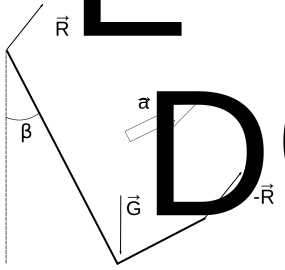
\includegraphics[width=0.45\linewidth]{./images/Vrijlichaamdiagram-1.png}
	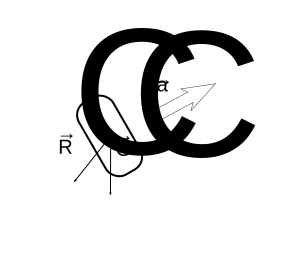
\includegraphics[width=0.45\linewidth]{./images/Vrijlichaamdiagram-2.png}
  \caption{Vrijlichaamsdiagramma van landingsgestel en wiel}
  \label{image:diagramma}
\end{figure}
Uit het vrijlichaamsdiagram van het landingsgestel volgt volgend krachtenevenwicht:
\begin{equation}
\begin{split}
-\vec{R}_{c}+\vec{G}_{d}+\vec{R}_{b} &= m_{l} \cdot \vec{a}_{d}\\
&=
\end{split}
\label{eq:dyn2.5}
\end{equation}
\subsection{Opgave 4}
\subsection{Opgave 5}

\end{document}
